\chapter{Our Approach}\label{cap:our_approach}

In Chapter \ref{cap:gld} we present the \textit{GLD} and argue why this distribution family is suitable to be used in UQ, while in Chapter \ref{cap:gld_clustering} we explore the possibility to use the $\lambda$ values of the \textit{GLD} to clustering uncertain data. Now in this Chapter we present a workflow to quantify the uncertainty in large-scale spatio-temporal models using the \textit{GLD}. In Chapter \ref{cap:gld_clustering} we present a solution to the \textbf{RQ.1}, in this Chapter we present a solution to the remaining four research questions.  

The rest of the Chapter is organized as follow: Section \ref{sec:dataflow} describes the proposed workflow and comment briefly the motivations to propose it and its steps. Section \ref{sec:fitting} presents the fitting step, that is divided into three sub-steps: the fitting process, \textit{GLD} validity check and the fitting process evaluation quality. Section \ref{sec:kriging} presents how to use spatio-temporal interpolation over the $\lambda$ values of the \textit{GLD} to estimate the uncertainty in spatio-temporal locations not previously analyzed (\textbf{RQ.2}). Section \ref{sec:clustering} discusses the integration of the clustering algorithm proposed in Chapter \ref{cap:gld_clustering} into the workflow. Section \ref{sec:queries} presents how to use the previous results to answer queries that arise in the UQ context, such us those queries we formulate in Chapter \ref{cap:intro} (\textbf{RQ.3, RQ.4 and RQ.3}).  
Section \ref{sec:suq2} presents an implementation of the proposed workflow in an R package named Simulation Uncertainty Quantification Querying (SUQ$^2$). Finally Section \ref{sec:approach_summary} summarize the Chapter.  

\section{UQ Proposed Dataflow}\label{sec:dataflow}
The proposed workflow to uncertainty quantification in \textbf{LSSTM} based on the \textit{GLD}, is divided into four steps, Figure \ref{fig:workflow}. The first step is the \textbf{fitting process}, where we implement algorithms to estimate the parameters of the \textit{GLD} that best fit the dataset at each spatio-temporal location. The second step is the \textbf{spatio-temporal interpolation (kriging)}. This step is included because in UQ is common to estimate the uncertainty (e.g. low order statistical moments, such as the standard deviation) in some points and then interpolate the uncertainty to other points. Analogously, we propose to do the same but using the $\lambda$ values of the \textit{GLD}. The third step is c\textbf{lustering uncertain data}, using the algorithm proposed and tested in Chapter \ref{cap:gld_clustering}. And finally the fourth is the \textbf{queries} step, where we expose how the results produced in the previous steps help us to answer queries that arise in the UQ context.

In the next sections we detail each of the UQ processing steps.

\begin{figure}[H]
    \centering
    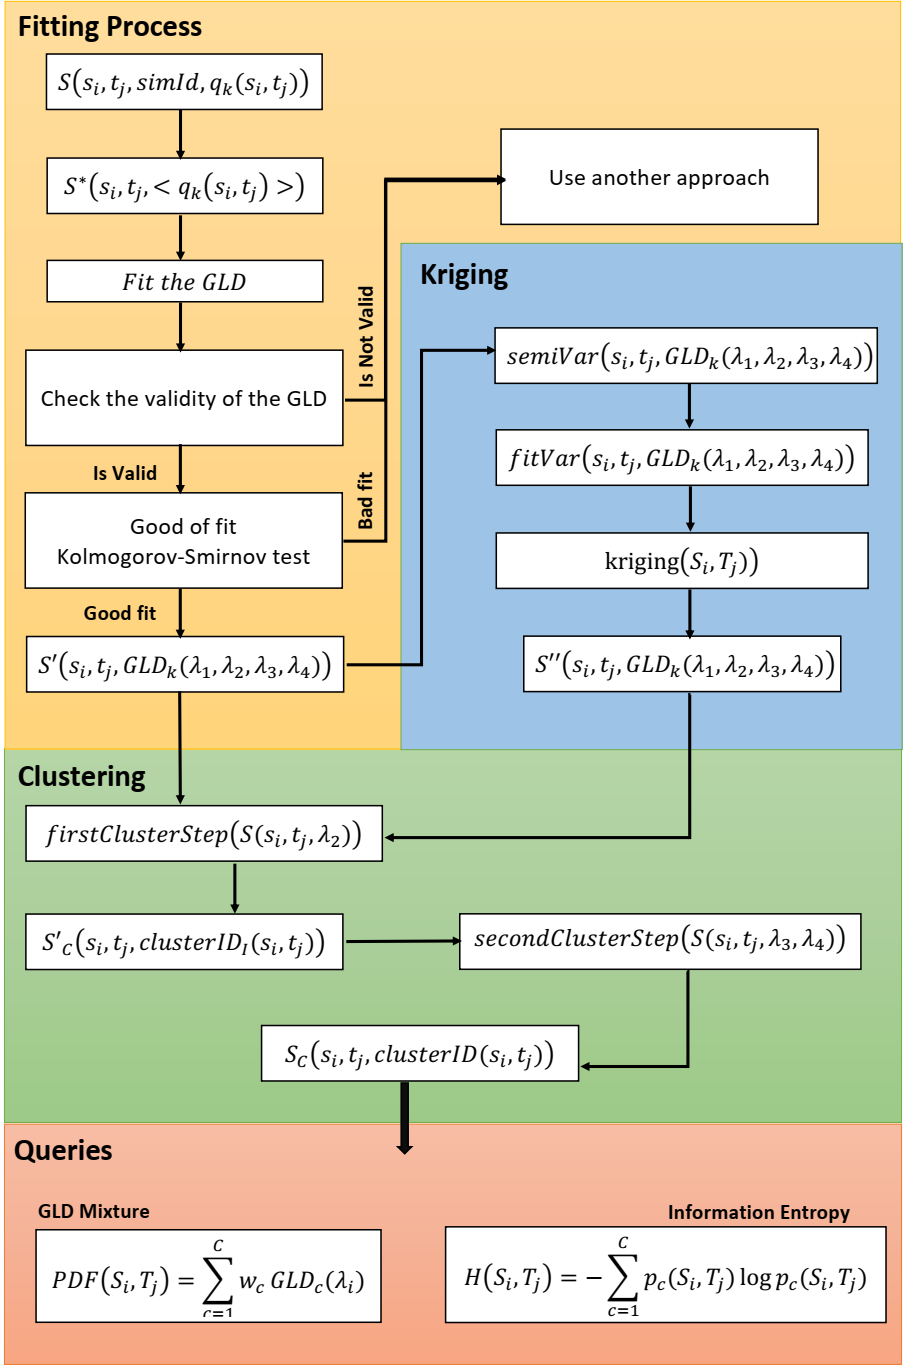
\includegraphics[width=0.8\textwidth]{img/Workflow.png}
    \caption{Proposed workflow. The workflow was divided in four steps, (i) the fitting process, (ii) the spatio-temporal interpolation (kriging), (iii) the clustering of the GLDs and, (iv) the queries over the results of the clustering process.}
    \label{fig:workflow}
\end{figure}

\section{Fitting a GLD to a spatio-temporal dataset}\label{sec:fitting}
In the more general case, the computational model $\bm{q}=\mathcal{M}(\bm{\theta})$ represents the spatio-temporal evolution of a complex systems, and the \textit{QoI} $\bm{q}$ could be represented as:  

\begin{equation} \label{eq:spatio_temporal}
\mathbf{Q} = (\mathbf{q}(s_{1},t_{1}),\mathbf{q}(s_{2},t_{2}),...,\mathbf{q}(s_{n},t_{n}))  
\end{equation}
where:
\begin{itemize}
\item $(s_{1},t_{1}),(s_{2},t_{2}),....,(s_{n},t_{n}) \in \mathcal{S} \times \mathcal{T}\subseteq\mathbb{R}^{3}\times\mathbb{R}$ represents a set of distinct spatio-temporal locations, and
\item $\mathbf{q}(s_{i},t_{j})$ represents a value of the \textit{QoI} at the spatio-temporal location $(s_{i},t_{j})$
\end{itemize}
%We could have many \textit{QoI}, but for simplicity here we are going to considere just one.

In the presence of a stochastic problem, at each spatio-temporal location $(s_{i},t_{j})$, we have many realizations of $q(s_{i},t_{j})$. A data set schema to represent this information can be modeled as (see also \ref{eq:data_base_structure}):
\begin{equation}
S(s_{i},t_{j},simId,q(s_{i},t_{j}))
\end{equation}
where $simId$ represents the \textit{id} of one simulation (realization).

The first step of our approach consists in find the \textit{GLD} that best fits our simulations on each spatio-temporal location. This step is divided in three minor tasks:
\begin{itemize}
\item Fit the \textit{GLD} to the data.
\item Evaluate the validity of the resulting \textit{GLD} on each spatio-temporal location.
\item Perform a ks-test to evaluate the quality of the fit on each spatio-temporal location.
\end{itemize}

The fitting process has been implemented following Algorithm \ref{alg:fitGLD}. Before starting the fitting process, we group all the simulations that correspond to the same spatio-temporal location $(s_{i},t_{j})$.  As a result, a new dataset with the following data schema is created: $\ S^*(s_{i},t_{j},<q_1,q_2,..,q_n>)$, where $q_i, 1 \le i \le n$, represents a vector holding all the values of $q$ at point $(s_{i},t_{j})$.

\subsection{The Fitting process}
\label{gldFitProcess}
Having prepared the dataset with the distribution at each spatio-temporal location, we are in conditions to process the GLD fitting step. Thus,for each spatio-temporal location $(s_{i},t_{j}) \in \mathcal{S} \times \mathcal{T}$ we apply a fitting function provided by the GLDEX R package described in section \ref{sec:gldex}. The lattter fits the \textit{GLD} to a vector $<q_1,q_2,..,q_n>$, line 2 of Algorithm \ref{alg:fitGLD}. As a result of this task, we get the $\lambda$ values of the \textit{GLD} that best fit the dataset at each spatio-temporal location, Equation \ref{eq:S_GLD} (see also \ref{eq:multi_array3}).
\begin{equation}\label{eq:S_GLD}
S'(s_{i},t_{j},GLD(\lambda_{1}, \lambda_{2}, \lambda_{3}, \lambda_{4}))
\end{equation}

\subsection{GLD validity check}
As we mention in section \ref{sec:parameterizations} the \textit{GLD} is not always valid, it depends on the $\lambda_{3}$  and $\lambda_{4}$ values. The evaluation of the validity of the \textit{GLD} is straightforward, if $\lambda_{3}$  and $\lambda_{4}$ are in the gray regions of Figure \ref{fig:rs_regions} the \textit{GLD} is not valid, on the other case is valid.

The validity check is performed in line 3 of Algorithm \ref{alg:fitGLD}, and as a result we get:
\begin{equation}
S_{validity}(s_{i},t_{j},valid(s_{i},t_{j})),
\end{equation}
where:
\begin{equation}
 \label{eq:validitycheck}
  valid(s_{i},t_{j}) =
  \begin{cases}
    1 & \text{if GLD is valid in $(s_{i},t_{j})$} \\
    0 & \text{otherwise}
  \end{cases}
\end{equation}

\subsection{Quality of the fit}
\label{Quality of the fit}
Now at the remaining points, where the \textit{GLD} is valid, we need to evaluate how good is the fit. That is, we evaluate whether the \textit{GLD} (PDF) correctly describes the dataset. We use here the Kolmogorov-Smirnov test (KS-test). The KS-test  determines if two datasets differ significantly. In this case, these datasets are: the original dataset and a second one generated using the fitted \textit{GLD}. As a result, this test returns two values: a Kolmogorov-Smirnoff Distance (D); and a p-value, line 5 of Algorithm \ref{alg:fitGLD}. The distance D is the maximum distance between both cumulative density functions (CDF), as shown in Figure \ref{fig:D_distance}. A small distance means that both, the dataset and the fitted PDF, are similar. 

\begin{figure}[ht]
    \centering
    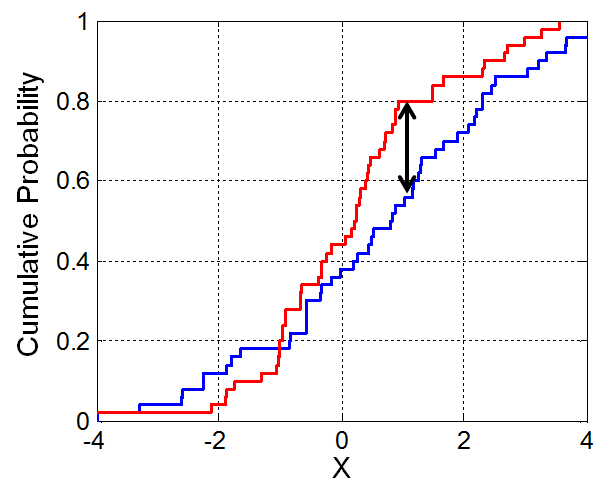
\includegraphics[width=0.8\textwidth]{img/D_distance.png}
    \caption{Illustration of the two-sample Kolmogorov–Smirnov statistic. Red and blue lines each correspond to an empirical distribution function, and the black arrow is the two-sample KS statistic.}
    \label{fig:D_distance}
\end{figure}

The second value, the p-value, is a more robust test, as it helps us to determine the significance of our results. Suppose we have two hypotheses, the null hypothesis  is that our PDF is a good fit to our dataset, and the alternative hypothesis  is that it is not. Then, a small p-value (typically $\leq 0.05)$ indicates strong evidence against the null hypothesis, so you reject the null hypothesis. A large p-value $(> 0.05)$ indicates weak evidence against the null hypothesis, so you fail to reject the null hypothesis. p-values very close to the cutoff (0.05) are considered to be marginal (could go either way). 

At the end of this task we have two new multidimensional arrays with the values of $\mathcal{D}$ and \textit{p}-value at each spatio-temporal locations.
\begin{equation}
S_{\mathcal{D}}(s_{i},t_{j},\mathcal{D}(s_{i},t_{j}))
\end{equation}
\begin{equation}
S_{p_{value}}(s_{i},t_{j},p_{value}(s_{i},t_{j}))
\end{equation}

Finally, in line 7 of Algorithm \ref{alg:fitGLD}, we store the $\lambda$ values of those \textit{GLDs} that are valid and return p-values greater than 0.05.

\begin{algorithm} 
\caption{Fitting the GLD to a spatio-temporal dataset}\label{alg:fitGLD}
\begin{algorithmic}[1] 
\Function{gldFit}{$S(s_{i},t_{j},<q_1,q_2,...,q_n>)$} 
\State $<\lambda_{1},\lambda_{2},\lambda_{3},\lambda_{4}> \gets \Call {fit.gld.lm}{<q_1,q_2,...,q_n>}$

\State $isValid_{(s_{i},t_{j})} \gets \Call {validityCheck}{<\lambda_{3},\lambda_{4}>}$
\If{$isValid_{(s_{i},t_{j})}$}
\State $[pvalue,D]_{(s_{i},t_{j})} \gets \Call{ks}{<\lambda_{1},\lambda_{2},\lambda_{3},\lambda_{4}>_{(s_{i},t_{j})}}$
\EndIf
\If{$pvalue_{(s_{i},t_{j})} > 0.05$}
\State $\Call{storeLambdas}{<\lambda_{1},\lambda_{2},\lambda_{3},\lambda_{4}>,s_{i},t_{j}}$
\EndIf
\EndFunction 
\end{algorithmic} 
\end{algorithm} 

\section{Spatio-Temporal Interpolation}\label{sec:kriging}
Although our interest is to quantify the uncertainty at each spatio-temporal locations, this is a timely and computationally prohibitive task. Neither the \textbf{GLD} or simpler approaches, as the evaluation of low order statistical moments, can be computed over the whole output space. Usually researchers place control points at particular points of interest, and then interpolate the uncertainty to other points as needed.

Spatial or temporal interpolation independently, are very well studies, and dozens of algorithms exist to compute new values by means of those methods. However, working with spatio-temporal domain implies that variability in space and time must be modelled, which is more complicated than modelling purely spatial or purely temporal variability \cite{Graler2016}.

Our purpose here is not to provide a new interpolation method over the \textbf{GLDs} $\lambda$ values, but show how spatio-temporal interpolation can be used to answer the \textbf{RQ.2}:
\begin{tcolorbox}
\textbf{RQ2.} what is the uncertainty in some spatio-temporal locations not previously analyzed?
\end{tcolorbox}

For this reason we select the state-of-the-art spatio-temporal interpolation method, from the best of our knowledge, proposed by Graler et al. in \cite{Graler2016}, and implemented it in the R package \textbf{gstat}. The selection obeys the fact that this implementation includes time as an extra dimension, and allows us to interpolate in space and time at the same time.

\subsection{Kriging over \textit{GLD}}
First to all, we define some concepts that are important to understand our proposal. The first concept is \textbf{what is Kriging?}.

\begin{defn}
Optimal interpolation based on regression against observed values of surrounding data points, weighted according to spatial covariance values.
\end{defn}

An the definition of \textbf{interpolation} is: 

\begin{defn}
Estimation of a variable at an unmeasured location from observed values at surrounding locations.
\end{defn}

For example, suppose we have a measure of the porosity at an spacial region, Figure \ref{fig:porosity}, and we want to estimate the porosity value in an unmeasured point marker with $+$ in the figure, based on porosity values at nearest six data points, Figure \ref{fig:kriging_example}. 

\begin{figure}[ht]
    \centering
    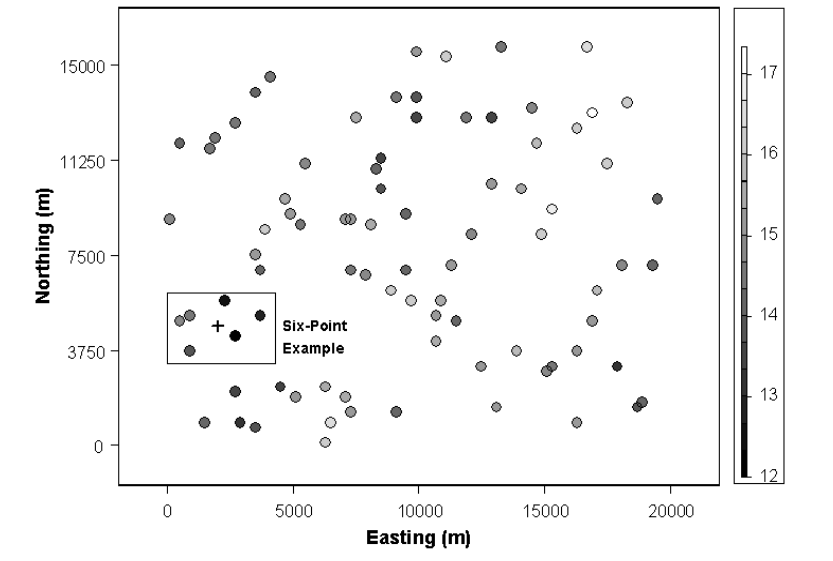
\includegraphics[width=0.8\textwidth]{mg/our_approach/porosity.png}
    \caption{Porosity measure over an spatial region. We want to estimate the porosity value in an unmeasured point marker with $+$.}
    \label{fig:porosity}
\end{figure}

\begin{figure}[ht]
    \centering
    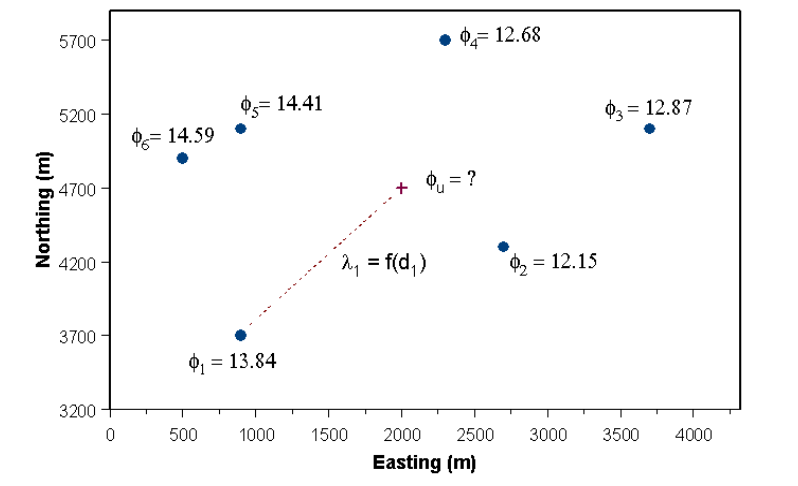
\includegraphics[width=0.8\textwidth]{mg/our_approach/kriging_example.png}
    \caption{Nearest six data points surrounding the point where we want to estimate the porosity.}
    \label{fig:kriging_example}
\end{figure}

All interpolation algorithms (inverse distance squared, splines, radial basis functions, triangulation, etc.) estimate the value at a given location as a weighted sum of data values at surrounding locations. Almost all assign weights according to functions that give a decreasing weight with increasing separation distance. Kriging assigns weights according to a (moderately) \textbf{data-driven weighting function}, rather than an arbitrary function, but it is still just an interpolation algorithm.

All kriging estimators are but variants of the basic linear regression estimator defined as:

\begin{equation}
Z(u*) - m(u) = \sum_{\alpha = 1}^{n(u)} \lambda_{\alpha}\left[Z(u_{\alpha} - m(u_{\alpha})) \right] 
\end{equation}

with:

\begin{itemize}
\item $\bm{u}, \bm{u_{\alpha}}$ location vectors for estimation point and one of the neighboring data points, indexed by $\alpha$,
\item $\bm{n(u)}$ number of data points in local neighborhood used for estimation of $Z(u*)$,
\item $\bm{m(u)}, \bm{m(u_{\alpha})}$ expected values (means) of $Z(u)$ and $Z(u*)$,
\item $\bm{\lambda_{\alpha}}$ kriging weight assigned to datum $Z(u_{\alpha})$ for estimation
location $u$; same datum will receive different weight for different estimation location
\end{itemize}

The goal is to determine weights, $\bm{\lambda_{\alpha}}$, that minimize the variance of the estimator

\begin{equation}
\sigma_{E}^2 = Var \lbrace Z*(u)-Z(u) \rbrace
\end{equation}

Kriging weights, $\bm{\lambda_{\alpha}}$, are derived from covariance function or semivariogram. The semivariogram is defined as:

\begin{equation}
\gamma(u_{i}, u_{j}) = \frac{1}{2}Var \lbrace Z(u_{i})-Z(u_{j}) \rbrace
\end{equation}

If two locations, $u_{i}$ and $u_{j}$, are close to each other, you expect them to be similar, so the difference in their values, $Z(u_{i})-Z(u_{j})$, will be small. As $u_{i}$ and $u_{j}$ get farther apart, they become less similar, so the difference in their values, $Z(u_{i})-Z(u_{j})$, will become larger.

There are different types of semivariograms, such as: circular, spherical, tetraspherical, exponential, Gaussian, etc.

The semivariogram provide information on the spatial autocorrelation of datasets. However, they do not provide information for all possible directions and distances. For this reason, and to ensure that kriging predictions have positive kriging variances, it is necessary to fit a model (in other words, a continuous function or curve) to the empirical semivariogram.

After you have uncovered the dependence or autocorrelation in your data and have finished with the first use of the data -using the spatial information in the data to compute distances and model the spatial autocorrelation- you can make a prediction using the fitted model. 

Summarizing, the kriging method is a process with three main steps (i) estimate the semivariogram, (ii) fit a model to the empirical semivariogram, and (iii) make predictions.

Those steps are implemented into the \textbf{gstat} R package. The implementation of this workflow over the \textbf{GLD} using \textbf{gstat} is shown in Algorithm \ref{alg:krigingGLD}. In line 2 the semivariogram is created, \textbf{gstat} provide different functions to create different semivariograms. In line 3 we fit a model using the dataset and the semivariogram. Finally in line 4 we make predictions of the $\lambda$ values of the \textit{GLDs} over the unmeasured regions.

\begin{algorithm} 
\caption{Spatio-temporal interpolation over the $\lambda_{(2,3,4)}$ values of the GLD.}\label{alg:krigingGLD}
\begin{algorithmic}[1] 
\Function{gldKriging}{$S(s_{i},t_{j}, <0,\lambda_{2},\lambda_{3},\lambda_{4}>)$} 
\State $gldModel \gets \Call {vgmST}{S(s_{i},t_{j},<0,\lambda_{2},\lambda_{3},\lambda_{4}>)}$
\State $fitGldVariogram \gets \Call {fit.StVariogram}{gldModel}$
\State $S''(s_{i},t_{j}) \gets \Call {krigeST}{fitGldVariogram, (\mathcal{S}_{i}, \mathcal{T}_{j})}$
\EndFunction 
\end{algorithmic} 
\end{algorithm} 

As a result of this algorithm a new dataset with the interpolated values of the \textbf{GLD} in the spatio-temporal locations not previously analyzed is returned, Equation \ref{eq:S_GLD_Kriging}. This strategy answers query \textbf{RQ2.} for the given spatio-temporal location.

\begin{equation}\label{eq:S_GLD_Kriging}
S''(s_{i},t_{j},GLD(\lambda_{1}, \lambda_{2}, \lambda_{3}, \lambda_{4}))
\end{equation}

%\emph{FP: VC PRECISA AO MENOS FORNECER UMA INTUIÇÃO DO ALGORITMO DE INTERPOLAÇÃO}

\section{GLD Clustering}\label{sec:clustering}
In Chapter \ref{cap:gld_clustering} we discussed how to use a \textit{GLD} to group uncertain data. Algorithm \ref{alg:clusterGLD2}, proposed in that chapter, is used here to provide the clustering of \textit{GLDs}.

\begin{algorithm} 
\caption{Clustering the GLD based on its $\lambda_{(2,3,4)}$ values.}\label{alg:clusterGLD2}
\begin{algorithmic}[1] 
\Function{gldClustering}{$S(s_{i},t_{j}, <0,\lambda_{2},\lambda_{3},\lambda_{4}>)$} 
\State $S(s_{i},t_{j}, clusterID_{I}) \gets \Call {firstClusterStep}{S(s_{i},t_{j},\lambda_{2})}$
\For{\textbf{each} $clId_{I}$}
\State $S(s_{i},t_{j}, clusterID_{II}) \gets \Call {secondClusterStep}{S(s_{i},t_{j},<\lambda_{3},\lambda_{4}>), S(s_{i},t_{j}, clusterID_{I})}$
\EndFor
\EndFunction 
\end{algorithmic} 
\end{algorithm} 

Algorithm \ref{alg:clusterGLD2} receives as an input the results of the previous steps, could be the outcome of the fitting process, Equation \ref{eq:S_GLD} or that of the kriging process Equation \ref{eq:S_GLD_Kriging}. The output of the algorithm is a dataset with schema where the cluster ids are associated to each GLD:
\begin{equation}
S_{\mathcal{C}}(s_{i},t_{j},GLD_{k},clusterID)
\end{equation}
where:
$clusterID$ represents the ID of the cluster to which the \textit{GLD} at the spatio-temporal location $(s_{i},t_{j})$ belongs to.

Once the dataset has been clusterized according to the \textit{GLD}, we can use this result to characterize the uncertainty in a particular spatio-temporal region, or to measure numerically the corresponding uncertainty. In subsections \ref{sub:gldMixtureWorkflow} and \ref{sub:InfomationEntropyRegionWorkflow}, we describe how those approaches are implemented (see Figure \ref{fig:workflow}).

\section{UQ Queries}\label{sec:queries}
In this section we discuss how UQ questions can be answered with the use of the UQ workflow. The following queries motivated in chapter 1 are discussed:

\begin{tcolorbox}
\textbf{RQ3.} what is the uncertainty at a specific spatio-temporal region? \\
\textbf{RQ4.} how to compare two regions as a function of their uncertainty? \\
\textbf{RQ5.} what is the least uncertain from a set of models?
\end{tcolorbox}

\subsection{Use of GLD mixture to characterize the uncertainty in an spatio-temporal region}
\label{sub:gldMixtureWorkflow}
Lets start with \textbf{RQ.3}. The naive algorithm to answer this question could be something as follow: given a spatio-temporal region $(\mathcal{S}_{i} \times \mathcal{T}_{j})$, read and analyze all the data generated during the simulation process on that region. This is a process current used by many researchers and proposed for example in provenance softwares. It is clear that this approach is not so efficient. Now, in our approach we first find the \textit{GLD} that best fits the dataset at each $(s_{i},t_{j})$, then we test whether the fit is a good one. As a \textit{GLD} is proved to be a good random variate generator (see Section \ref{sec:gld_random_variate}), then we can substitute the raw data by the associated \textit{GLD}. Next, in the clustering step, we group all the \textit{GLDs} by their similarities, and then we test if the centroid of each cluster statistically represent the remaining members of their cluster. If this condition is met, then is possible to substitute each \textit{GLD} by the centroid of the cluster it belongs to. At the end of this process we substitute the raw data by a few centroids of the clusters.
  
Now, coming back to the question: \textit{"what is the uncertainty at a specific spatio-temporal region $(\mathcal{S}_{i} \times \mathcal{T}_{j})$?"}, we can answer it looking to the centroids of the clusters.

In $(\mathcal{S}_{i} \times \mathcal{T}_{j})$ each cluster may be qualified with a weight given by (see also \ref{eq:validitycheck}):
\begin{equation}
w_{k}=\frac{1}{N}\sum_{i=1}^S \sum_{j=1}^T w(s_{i},t_{j})
\end{equation}
where:
\begin{equation}
  w(s_{i},t_{j}) =
  \begin{cases}
    1 & \text{if $clusterID(s_{i},t_{j}) = k$} \\
    0 & \text{otherwise}
  \end{cases}
\end{equation}
and  \textit{N} is the number of points in the region $(\mathcal{S}_{i} \times \mathcal{T}_{j})$.

The weight $w_k$ is the frequentist probability of occurrence of the cluster \textit{k} in the region, and complies with the conditions outlined in section \ref{sec:gld_mixture} that $w_{k} \geq 0$ and $\sum w_{k}=1$.

Remember that the mixture of the \textit{GLDs} can be written as:
\begin{equation}
f(x)=\sum_{k=1}^K w_{k}GLD(\lambda_{1},\lambda_{2},\lambda_{3},\lambda_{4})
\end{equation}
So, if we have the weights and a representative \textit{GLD} for each cluster, we have the mixture of \textit{GLD} that characterizes the uncertainty in the spatio-temporal region $(\mathcal{S}_{i} \times \mathcal{T}_{j})$.

The process to generate the mixture of \textit{GLDs} that characterizes the uncertainty on a region $(\mathcal{S}_{i} \times \mathcal{T}_{j})$ is presented in Algorithm \ref{alg:mixGLD}.

\begin{algorithm} 
\caption{GLD mixture in a region $(\mathcal{S}_{i} \times \mathcal{T}_{j})$}\label{alg:mixGLD}
\begin{algorithmic}[1] 
\Function{gldMixture}{$\mathcal{S}_{i} \times \mathcal{T}_{j}, C_{\mathcal{S}_{i} \times \mathcal{T}_{j}}$} 
%\State $K \gets \Call {clustersIn}{\mathcal{S}_{i} \times \mathcal{T}_{j}}$
\For{\textbf{each} $p_i$ in $(\mathcal{S}_{i} \times \mathcal{T}_{j})$}
\State $c \gets cluster(p_i)$
\State $w_c= w_c+1$
\State $N=N+1$
\EndFor
\State \textbf{end for}
\State \Return $\frac{1}{N} \sum_{c}^{C_{(\mathcal{S}_{i} \times \mathcal{T}_{j})}} 
    w_{c} * c.getGLD()$
\EndFunction 
\end{algorithmic} 
\end{algorithm} 

\subsection{Information Entropy as a measure of the uncertainty in an spatio-temporal region}
\label{sub:InfomationEntropyRegionWorkflow}
Another way to answer query \textbf{RQ.3} is using the Information Entropy (see Section \ref{subsub:informationentropytomeasuretheuncertainty}). In that section we highlight a limitation related to the fact that we need to know the possible outcomes of the system to use Information Entropy. In the cases where we can use the clusters  obtained in \ref{sec:clustering} as the different outcomes of the system, Information Entropy could be used as a measure of the uncertainty in an spatio-temporal region.
  
The equation \ref{eq: spatio-temporal Entropy} can be rewritten as follows:
\begin{equation}\label{eq: spatio-temporal EntropyWorkflow}
H(s,t)=-\sum_{c=1}^C p_{c}(s,t)\log p_{c}(s,t)
\end{equation}
where $c$ represents a particular cluster of the total number of clusters $C$, and $p_{c}(s,t)$ represents the probability of occurences of the cluster $c$ in the spatio-temporal region $(s,t)$.

Algorithm \ref{alg:informationEntropy}  computes the Information Entropy in a region $C_{(\mathcal{S}_{i} \times \mathcal{T}_{j})}$. In lines 2 to 7, we compute the probability of each cluster in the region, similar to section \ref{sub:gldMixtureWorkflow}. Using this probability we compute the Information Entropy $H(s, t)$, line 8, and finally we return the result in line 9.

\begin{algorithm} 
\caption{Information Entropy in a region $(\mathcal{S}_{i} \times \mathcal{T}_{j})$}\label{alg:informationEntropy}
\begin{algorithmic}[1] 
\Function{gldMixture}{$\mathcal{S}_{i} \times \mathcal{T}_{j}, C_{\mathcal{S}_{i} \times \mathcal{T}_{j}}$} 
%\State $K \gets \Call {clustersIn}{\mathcal{S}_{i} \times \mathcal{T}_{j}}$
\For{\textbf{each} $p_i$ in $(\mathcal{S}_{i} \times \mathcal{T}_{j})$}
\State $c \gets cluster(p_i)$
\State $w_c= w_c+1$
\State $N=N+1$
\EndFor
\State \textbf{end for}
\State $p_{c}(s,t)= \frac{w_c}{N}$
\State $H(s, t) \gets -\sum_{c=1}^C p_{c}(s,t)\log p_{c}(s,t)$
\State \Return $H(s, t)$
\EndFunction 
\end{algorithmic} 
\end{algorithm} 

The advantage of the Information Entropy, with respect to the GLD mixture approach, is that it synthesizes the uncertainty in a single comparable value.  

\subsection{Information Entropy and regions comparison}
Information Entropy can be used to answer other questions, such as: \textit{"\textbf{RQ4.} how to compare two regions as a function of their uncertainty?"}.  Its application here is straightforward, as it has been mentioned in Section \ref{InformationEntropy}, the Information Entropy is zero when we are certain and reaches a maximum value when the uncertainty is maximal, respectively. Then, if we want to compare two regions we compute the $H(s, t)$ for each one, and the region with the smaller value of $H(s, t)$ is the taken as the one presenting less uncertainty.  

\subsection{Information Entropy and model selection}
Similarly to the previous section, we can use Information Entropy to compare two models. Suppose we have a set of models $\mathcal{M} = \lbrace \mathcal{M}_{1}, \mathcal{M}_{2},...,\mathcal{M}_{n} \rbrace$ and we want to know what is the less uncertain in $(\mathcal{S}_{i} \times \mathcal{T}_{j})$. We proced to compute $H(s,t, \mathcal{M}_{i})$ for each model, and the one with smaller value of $H(s,t, \mathcal{M}_{i})$ is taken as the least uncertain in that region.

\subsection{Other queries}
Although in this section we present four different queries to answer three different questions (\textbf{RQ.3}, \textbf{RQ.4} and \textbf{RQ.5}), our approach leaves open the option to develop new queries to solve questions that arise in UQ context. In Section \ref{sec:use_case_II_queries}  we show how new queries can be answered quickly, thanks to the flexibility of this approach.

\section{SUQ$^2$ R package}\label{sec:suq2}
The proposed approach has been implemented as an R package named SUQ$^2$, an acronym of \textbf{S}imulation \textbf{U}ncertainty \textbf{Q}uantification \textbf{Q}uerying, freely available at \href{https://github.com/nmlemus/suq2}{SUQ$^2$}. As this package is in a development stage, to install it you need to install the R \textbf{devtools} package first and then use a function \textbf{install\_github} to install SUQ$^2$.

\begin{lstlisting}[language=r]
> install.packages("devtools")
> install_github("nmlemus/suq2")
\end{lstlisting}

The package has been divided into five sub-package, one for each step or the workflow and other one to show the results. The name of the sub-package are: \textbf{fit}, \textbf{kriging}, \textbf{clustering}, \textbf{queries} and \textbf{plot}.

As R is an interactive language, to warrant the easy to use of the functions inside the package we use the following pattern: (i) the name of all package fucntions start with \textbf{suq2.}; (ii) after \textbf{suq2.} we add a name that identifies a sub-package, for example the name of all the functions of the sub-package \textbf{plot} start with \textbf{suq2.plot.}; (iii) and finally a name that identifies the functionality of the function. For example a function to plot a gld based on its $\lambda$ values is named \textbf{suq2.plot.gld()}, while a function to cluster the \textit{GLDs} based on $\lambda_{2}$ is \textbf{suq2.clustering.lambda2()}.

The full documentation of the package is available inside the installation and in Appendix A.

\section{Summary}\label{sec:approach_summary}
In this Chapter we present the workflow of the proposed approach. The workflow is divided into four steps: fitting, kriging, clustering and queries. The algorithms of all the steps are presented and commented. In Section \ref{sec:queries} the queries to answer the research questions raised in the introduction were discuss. Finally, in Section \ref{sec:suq2} we present SUQ$^2$, an R package that implements our approach.  